\chapter[Manual do jogo]{Manual do jogo}
O jogo é composto em 2 pacotes, o pacote de exercícios e o pacote de estatísticas.

É na página inicial que você pode escolher o que deseja fazer.

\begin{figure}[H]
\centering
\caption{Tela inicial}
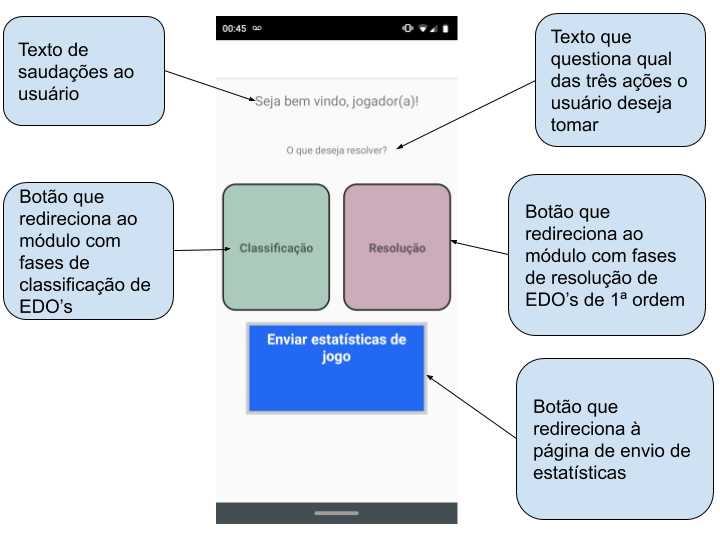
\includegraphics[scale=0.72]{figuras/tela_inicial.png}

\small{Fonte: do próprio autor}
\end{figure}


\section[Pacote 1 - Jogo]{Pacote 1 - Jogo}
No pacote de exercícios temos dois módulos, o de classificação e o de resolução.

\subsection[Módulo 1: Classificação]{Módulo 1: Classificação}
O módulo de classificação objetiva fixar o reconhecimento e a classificação de EDs. Este é composto de seis fases: tipo, ordem, homogeneidade, linearidade, separável e exata. Essas fases foram classificadas como sendo da mais fácil para a mais complexa. Para navegar entre as fases basta arrastar a tela para a direita.
Cada fase tem o domínio das suas perguntas e o número fixo de 20 equações que são selecionadas aleatoriamente de acordo com a fase.

As perguntas de tipo são: 
\begin{itemize}
	\item{}Escolha a ED ordinária
	\item{}Escolha a ED parcial
\end{itemize}


As perguntas de ordem são:
\begin{itemize}
	\item{}Escolha a ED de ordem 1
	\item{}Escolha a ED de ordem 2
	\item{}Escolha a ED de ordem 3
	\item{}Escolha a ED de ordem superior
\end{itemize}
 	

As perguntas de homogeneidade são:
\begin{itemize}
	\item{}Escolha a ED homogênea
	\item{}Escolha a ED NÃO homogênea
\end{itemize}
					
 
As perguntas de linearidade são:
\begin{itemize}
	\item{}Escolha a ED linear
	\item{}Escolha a ED NÃO linear
\end{itemize} 

As perguntas para a fase separável são:
\begin{itemize}
	\item{}Escolha a ED separável
	\item{}Escolha a ED NÃO separável
\end{itemize}

As perguntas se exata são:
\begin{itemize}
	\item{}Escolha a ED exata
	\item{}Escolha a ED NÃO exata
\end{itemize} 

\begin{figure}[H]
\centering
\caption{Modo de classificação parte 1}
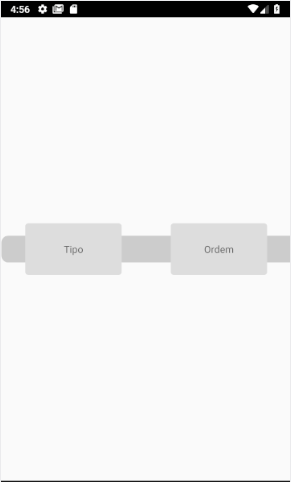
\includegraphics[scale=0.52]{figuras/modo_classificacao_1.png}
\end{figure}

\begin{figure}[H]
\centering
\caption{Modo de classificação parte 2}
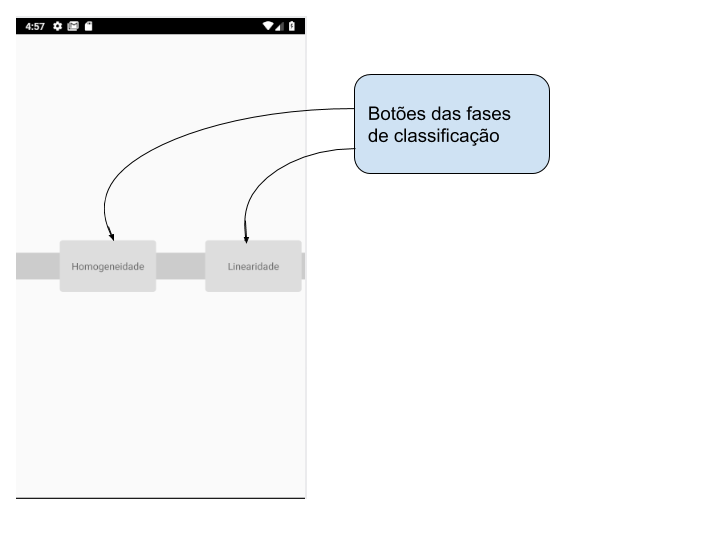
\includegraphics[scale=0.52]{figuras/modo_classificacao_2.png}
\end{figure}

\begin{figure}[H]
\centering
\caption{Modo de classificação parte 3}
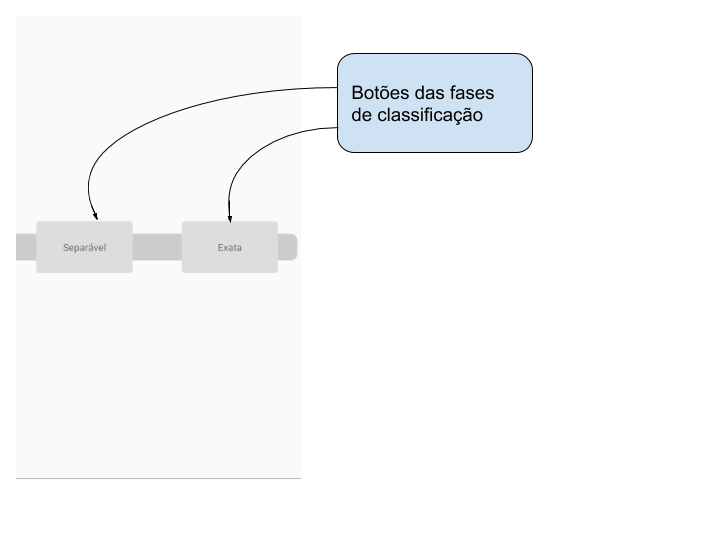
\includegraphics[scale=0.52]{figuras/modo_classificacao_3.png}
\end{figure}

As fases de classificação apresentam quatro equações como opção sendo que apenas 1 é a correta.
Ao pressionar cada opção por um tempo aparecerá a imagem da equação em uma janela modal para tentar melhorar a visualização.
Para escolher uma opção basta dar um toque na opção desejada.
Em caso de acerto da equação carregará automaticamente a próxima pergunta.
Em caso de erro aparecerá o \textit{feedback} da escolha da opção inválida.
Ao fim da fase será redirecionado novamente para o modo de classificação, após a parabenização do jogador, onde é possível escolher outra fase para jogar ou voltar para trocar o módulo.

\begin{figure}[H]
\centering
\caption{Exemplo da fase de classificação de homogeneidade}
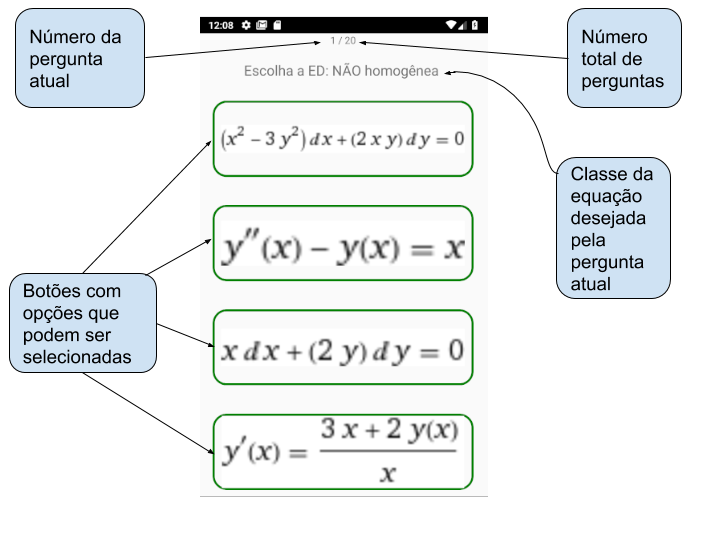
\includegraphics[scale=0.52]{figuras/ex_ed_n_homog.png}
\end{figure}

\begin{figure}[H]
\centering
\caption{Exemplo da fase de classificação de tipo}
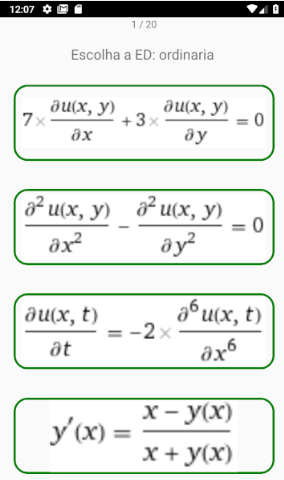
\includegraphics[scale=0.52]{figuras/ex_ed_ordinaria.png}
\end{figure}

\begin{figure}[H]
\centering
\caption{Feedback fornecido à uma tentativa inválida}
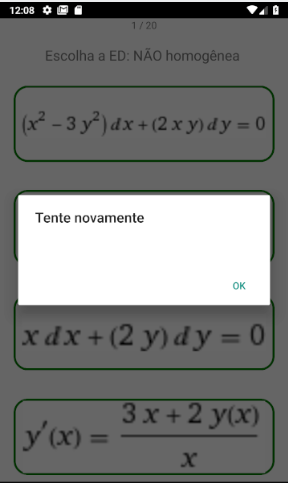
\includegraphics[scale=0.52]{figuras/tente_novamente.png}
\end{figure}

\begin{figure}[H]
\centering
\caption{Tela de finalização do modo de classificação}
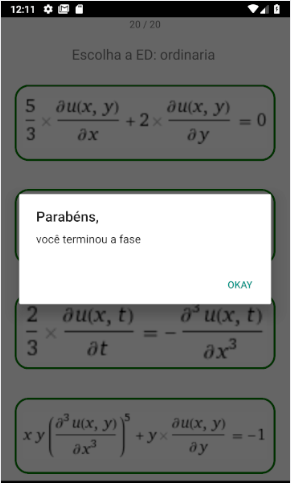
\includegraphics[scale=0.52]{figuras/fim_fase.png}
\end{figure}

\subsection[Módulo 2: Resolução]{Módulo 2: Resolução}

O módulo de resolução visa fixar o conhecimento de resolução de EDOs de 1ª e tem quatro fases. Sendo elas homogênea, NÃO homogênea, exatas e NÃO exatas. Neste módulo estão presentes APENAS equações diferenciais ordinárias de primeira ordem que contenham respostas. 

\begin{figure}[H]
\centering
\caption{Modo de resolução parte 1}
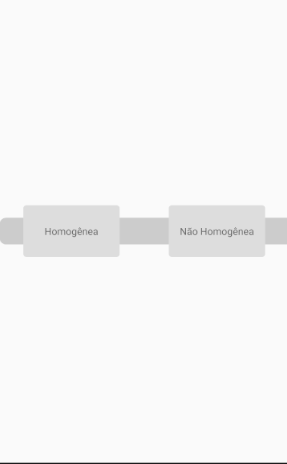
\includegraphics[scale=0.52]{figuras/modo_resolucao_1.png}
\end{figure}

\begin{figure}[H]
\centering
\caption{Modo de resolução parte 2}
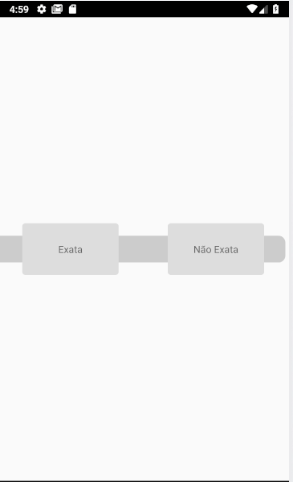
\includegraphics[scale=0.52]{figuras/modo_resolucao_2.png}
\end{figure}


O módulo de resolução trata-se de um jogo da memória, o qual tem o objetivo de encontrar as cartas gêmeas. Uma carta contém a EDO proposta e a carta gêmea contém a solução correta para a equação proposta.

Existem dois campos reservados na tela para mostrar as cartas selecionadas. O jogo é composto de vinte cartas (dez EDOs e dez soluções, uma de cada EDO). Cada carta é selecionada com um toque sobre ela, onde sua face será mostrada e seu conteúdo se mostrará em um dos dois campos reservados. Cada clique inverte o lado da carta que está sendo mostrado. Ao selecionar duas cartas haverá a comparação se são complementares (ou seja, pergunta e resposta). Em caso afirmativo, as cartas congelarão não sendo mais possível interagir com elas, em caso negativo apenas esconderão sua face para que inicie outra tentativa do jogador.

\begin{figure}[H]
\centering
\caption{Jogo da memória com 1 carta selecionada}
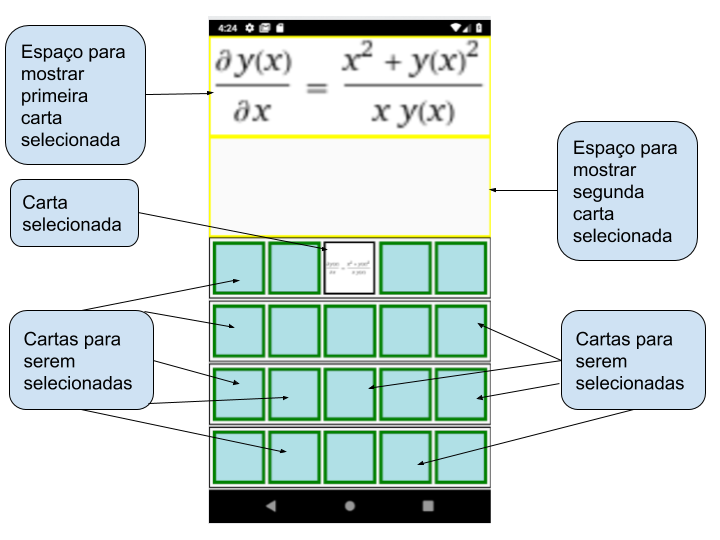
\includegraphics[width=\textwidth,height=\textheight,keepaspectratio]{figuras/resolucao_1imagem.png}
\end{figure}

\begin{figure}[H]
\centering
\caption{Jogo da memória com alguns pares encontrados}
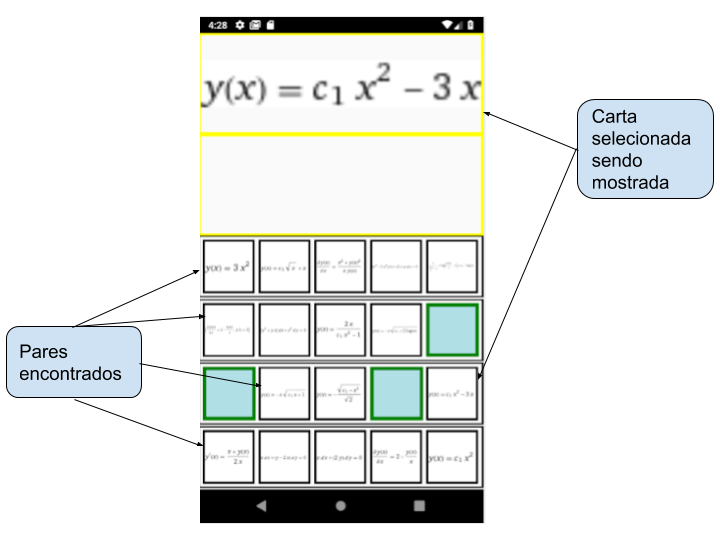
\includegraphics[width=\textwidth,height=\textheight,keepaspectratio]{figuras/resolucaoCartasAcertadas.png}
\end{figure}

\begin{figure}[H]
\centering
\caption{Vitória de jogo da memória}
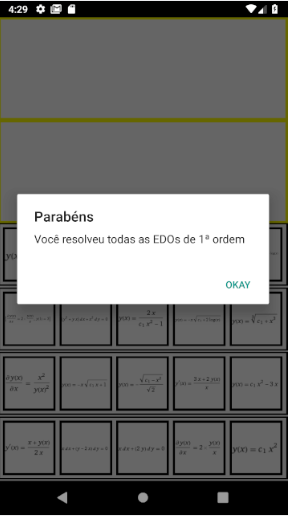
\includegraphics[scale=0.72]{figuras/resolucao_fim.png}
\end{figure}

Ao terminar qualquer fase do jogo da memória, após a confirmação o jogo retornará à tela de seleção da fase a ser jogada.

\begin{comment}
\subsection[Módulo 3]{Módulo 3}
– Jogo de classificação, perguntar técnica de resolução a ser utilizada em cada equação.

\end{comment}


\section[Pacote 2]{Pacote 2}
O pacote de estatísticas está relacionado à coleta de dados para a avaliação da quantidade de erros nas questões, quais foram as questões mais erradas e qual fase os estudantes tem mais dificuldade. O envio das estatísticas para o servidor não ocorrerá de forma programada, depende do jogador enviar os dados de acordo com a sua vontade de colaboração através de um botão e a confirmação do envio.


Na tela principal do jogo, terá um botão para enviar sugestões do jogo e outro botão para notificar erros e bugs encontrados.
O botão de enviar sugestões de jogo redirecionará a uma tela onde o jogador pode escrever x caracteres de sugestões e confirmar o envio para enviar ao servidor central de análise, essas sugestões podem se tornar \textit{issues} e/ou \textit{features} novas do jogo.
O botão de erros e bugs encontrados redirecionará a uma nova tela onde é possível escrever e/ou anexar 1 foto do incidente ocorrido, para que este possa ser analisado.

\begin{comment}
No desafio do modo de jogo 1, o jogador corre contra o tempo para classificar o maior número de equações de possíveis. A cada 3 respostas consecutivas corretas serão adicionados 2 segundos de tempo. Ao fim do desafio ficará registrado o récorde de pontuação do jogador.

Na fase 2 que é o jogo da memória o jogador lidará com problemas de resolução de exercícios.
Uma carta é uma equação e a sua carta gêmea é a resposta da equação.
No início existem menos cartas e exercícios mais fáceis, conforme prossegue no nível de dificuldade aumentarão o número de cartas e a dificuldade dos exercícios.

No desafio do modo de jogo 2, é o jogo da memória ao inverso, todas as cartas mostram os seus valores   e ao clicar na carta ela vira de lado mostrando o desenho da estampa da carta. O objetivo a ser atingido é esconder o valor de todas as cartas sem cometer nenhum tropeço errando a combinação de pares. Ao fim do desafio ficará registrado a quantidade récorde do mínimo de tropeços do jogador.

No modo 3 o jogo será em terceira pessoa, o jogador estará imerso no labirinto ao invés de 2D (visão superior) igual o modo de jogo 1 e 2. Neste modo o jogador possui um avatar que pode se locomover pelo labirinto. O labirinto possui mais de uma maneira de chegar à saída, porém existem caminhos mais longos que outros. No labirinto os jogadores irão se deparar com problemas no caminho, onde precisarão resolver problemas de aplicações para poder passar. A vantagem do labirinto é que existe mais de um caminho para chegar ao fim e o jogador pode escolher outro caminho caso não esteja satisfeito com o primeiro escolhido. As questões de aplicação serão a respeito de crescimento de bactérias atrapalhando o caminho, trajetórias de projeteis lançados no jogador, escoamento de fluidos, transferência de calor para derretimento de barreiras.


Requisitos do jogo: \\
Responsivo; \\
\textit{Feedbacks} constantes ao fim de atividades com redirecionamento às próximas ações; \\
Instruções iniciais com pequenas etapas; \\
Complexidade das instruções devem ser progressivas; \\
Confirmação do objetivo esperado na atividade; \\
Variação das atividades para evitar cansaço; \\
Diversidade de itens para pessoa escolher o desejado.

\end{comment}

